\section{Ausgesuchte Systeme}
\label{sec:Ausgesuchte Systeme}

Zwei der sechs Systeme im \cref{sec:CRS-Git} werden aufgrund deren Eigenschaften, die in der Firma benötigt sind, aufgebaut und getestet. Diese Sind Bitbucket \cref{subsec:Bitbucket} und Gerrit \cref{subsec:Gerrit}.
Folgende Punkte werden beim Testen betrachtet:
\begin{itemize}
	\item Wie aufwendig der Systems Aufbau ist
	\item Wie kann der Review gestartet und geschlossen werden
	\item Kann eine Pull-Request im Vergleich zu den anderen Methoden des Reviews vorteilhaft sein
	\item Erfüllt das System die Kriterien im \cref{sec:kriterien}
\end{itemize}

Nach der Testphase werden die zwei Systeme ausgewertet, miteinander verglichen und deren Vor- und Nachteile vorgestellt.

\section{Testphase}
\label{sec:testphase}

Zum Testen vom Reviews Workflow und von anderen Funktionen der ausgesuchten Systeme \cref{sec:Ausgesuchte Systeme}, wird diese Arbeit, die bereits mit Git versioniert und auf dem Server (Namens odin) der Software-Abteilung gehostet wurde, verwendet, deswegen wird sie in den nächsten Bildern erscheinen.  Die zwei Systeme werden ebenfalls auf odin installiert, wohl wissend, dass auf odin ein Debian läuft. Und Der Reviewer wird Björn schäpers \cite{Bjoern} sein.

\subsection{Bitbucket}
\label{subsec:Test_Bitbucket}

In den folgenden Unterabschnitten werden die Varianten:
\begin{itemize}
	\item Bitbuckets Webanwendung. Hosten auf Bitbuckets Server
	\item Self-hosten mit Bitbucket-Server
\end{itemize}

vorgestellt und miteinander verglichen.

\subsubsection{Hosten auf dem Server des Anbieters}
\label{subsubsec:Bitbucket-Cloud}

Für den Beginn Verlangt die Webanwendung vom Bitbucket nur eine Anmeldung und schon kann man anfangen, Projekte zu erstellen, in denen die Repositories geklont oder neue erstellt werden können. In dieser Anwendung können auch Funktionen durchgeführt werden, die man mit dem Command Line von Git macht. Wie beispielsweise ein neues Branch erstellen, wie in der \cref{fig:Bitbucket-Branch-erstellen} zu sehen ist oder ein Repositpry klonen.

\begin{figure}[H]
	\centering
	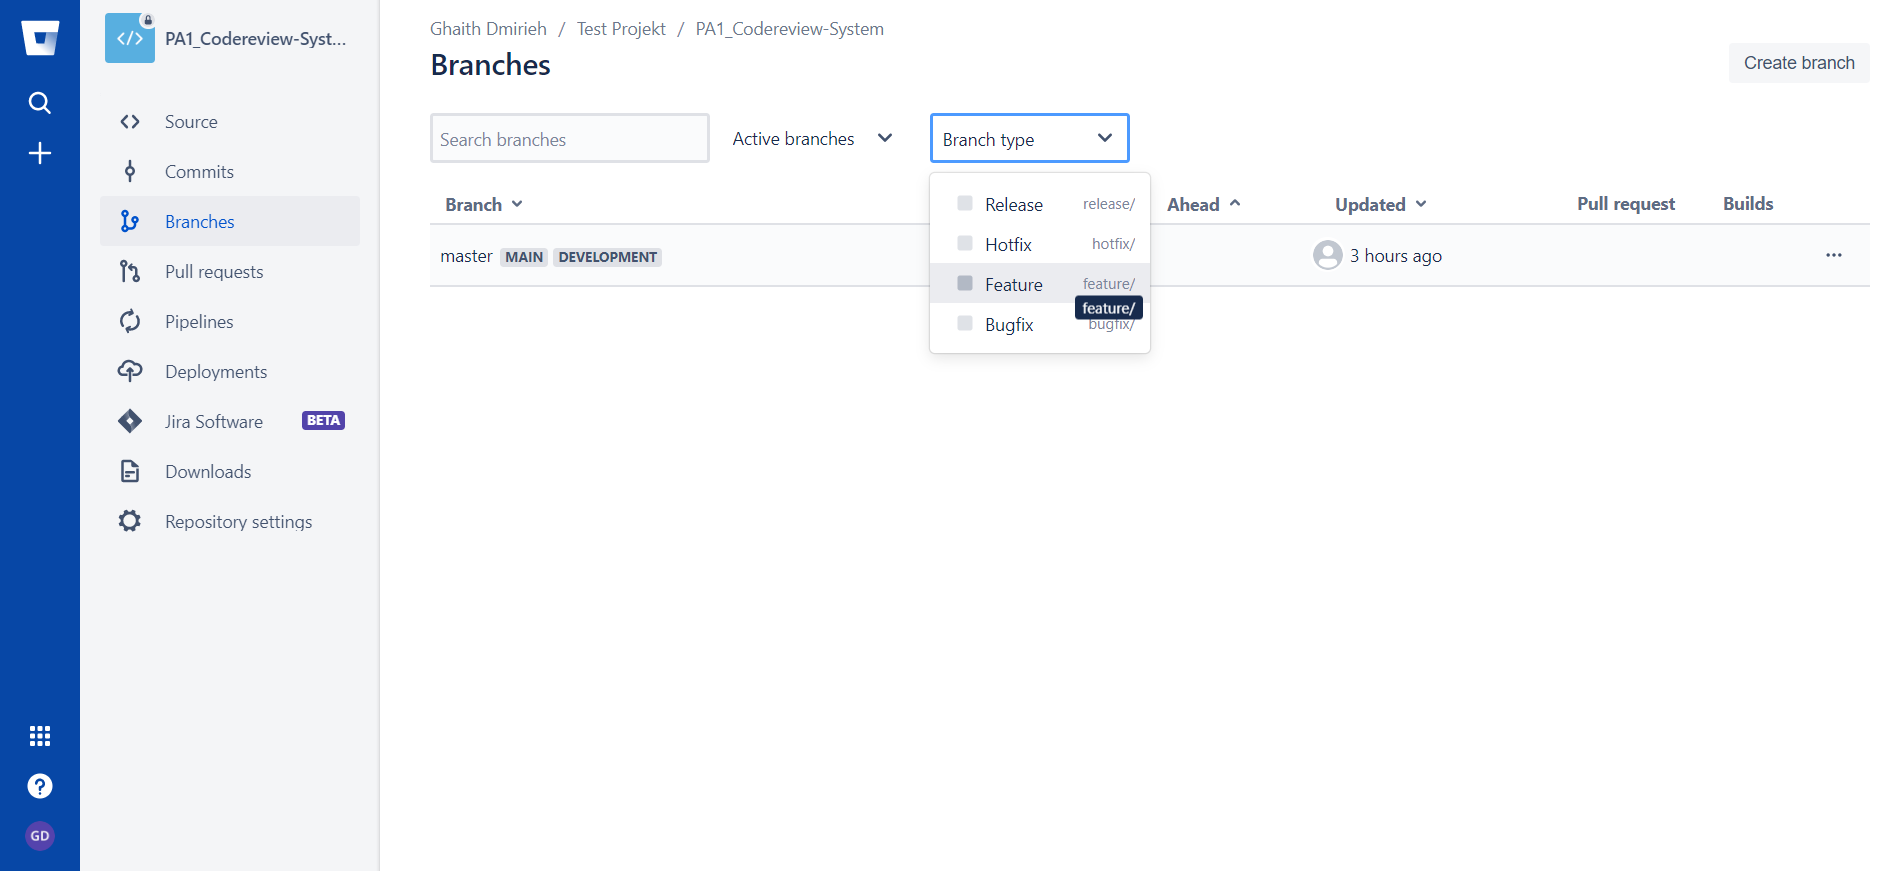
\includegraphics[width=1.0\textwidth]{Bitbucket-Branch-erstellen}
	\caption[Branch auf Bitbuckets Anwendung erstellen]{Ein neues Branch erstellen\\Eigenes Screenshot}
	\label{fig:Bitbucket-Branch-erstellen}
\end{figure}

Die Webanwendung ist imstande, die Änderungsvergleich von jedem commit sowohl inline als auch side-by-side anzuzeigen. Ein Beispiel dafür ist die \cref{fig:Diffs_side-by-side}.

\begin{figure}[H]
	\centering
	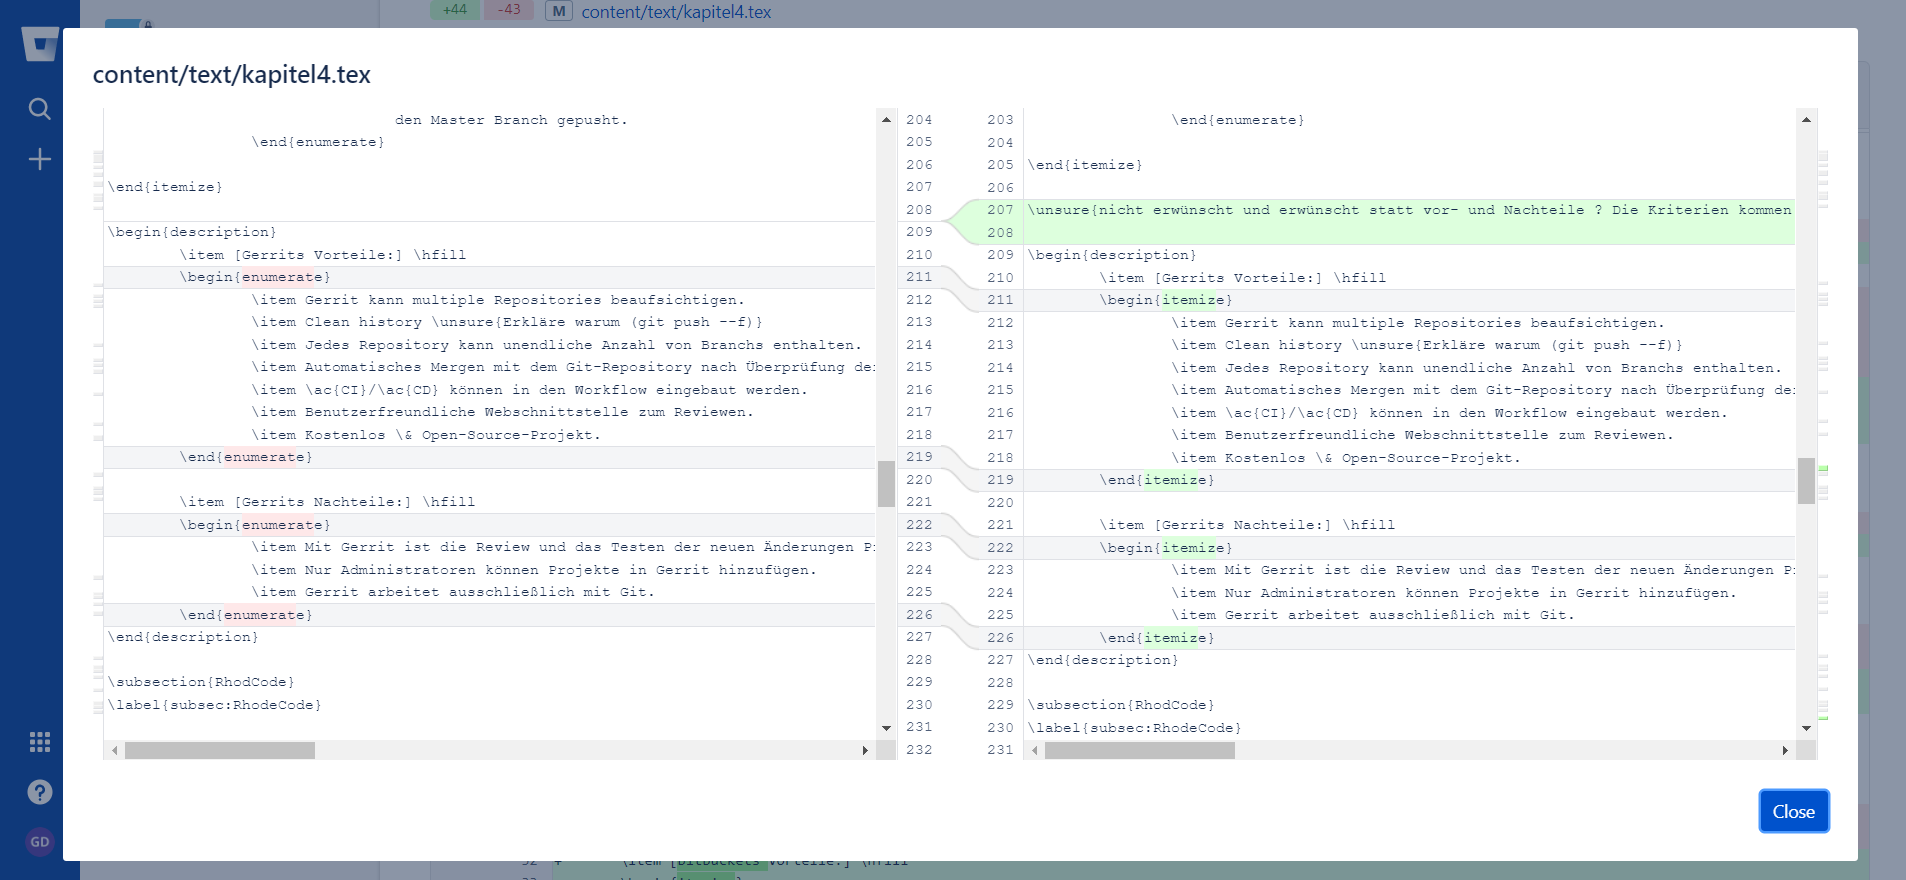
\includegraphics[width=1.0\textwidth]{Bitbucket side-by-side diffs}
	\caption[Bitbuckets Webanwendung side-by-side Änerungsvergleich]{Diffs side-by-side\\Eigenes Screenshot}
	\label{fig:Diffs_side-by-side}
\end{figure}

Im Gegensatz zu anderen Tools wird hier nur die Stelle, die geändert ist, markiert und nicht die ganze Zeile, die dazu gehört, was bei einer klaren Übersicht beiträgt.

\textbf{Pull-Request:} \unsure{1. klone das repository vom Bitbucket\\2. Erstelle ein Feature-Branch\\3. Füge Die Änderungen im Abschnitt 5 hinzu\\6. sende die Pull-Anfrage an Björn}

\subsubsection{Self-Hosten}
\label{subsubsec:Bitbucket-self-host} 

\subsection{Gerrit}
\label{subsubsec:Test_Gerrit}

Bei Gerrit handelt es sich nur um Self-Hosten \dots

\subsection{Vergleich}
\label{subsec:Vergleich_Bitbucket_Gerrit}

\unsure{Die Vergleichstabelle soll detaillierter sein}

\subsection{Auswertung}
\label{subsec:Auswertung}
